We use \mll~and \mt~to construct 2D templates. Exact definitions of 
them are as follows.  

%
\begin{itemize}
\item the dilepton mass $\mll$;
\item transverse Higgs mass, 
$\mt^{\ell\ell\met} = \sqrt{2\pt^{ll}\met(1-cos(\Delta\phi_{\ell\ell-\met}))}$ where 
$\Delta\phi_{\ell\ell-\met}$ is the angle between dilepton
direction and \met in the transverse plane.
\end{itemize} 

Figure~\ref{fig:templates_125_ex} shows 2D templates for 
signal at \mHi = 125 \GeV~(left) and \qqww (right).

%
\begin{figure}[!hbtp]
	
	%
	\centering
	\subfigure[Signal]{
	\centering
	\label{subfig:template_signal_125}
		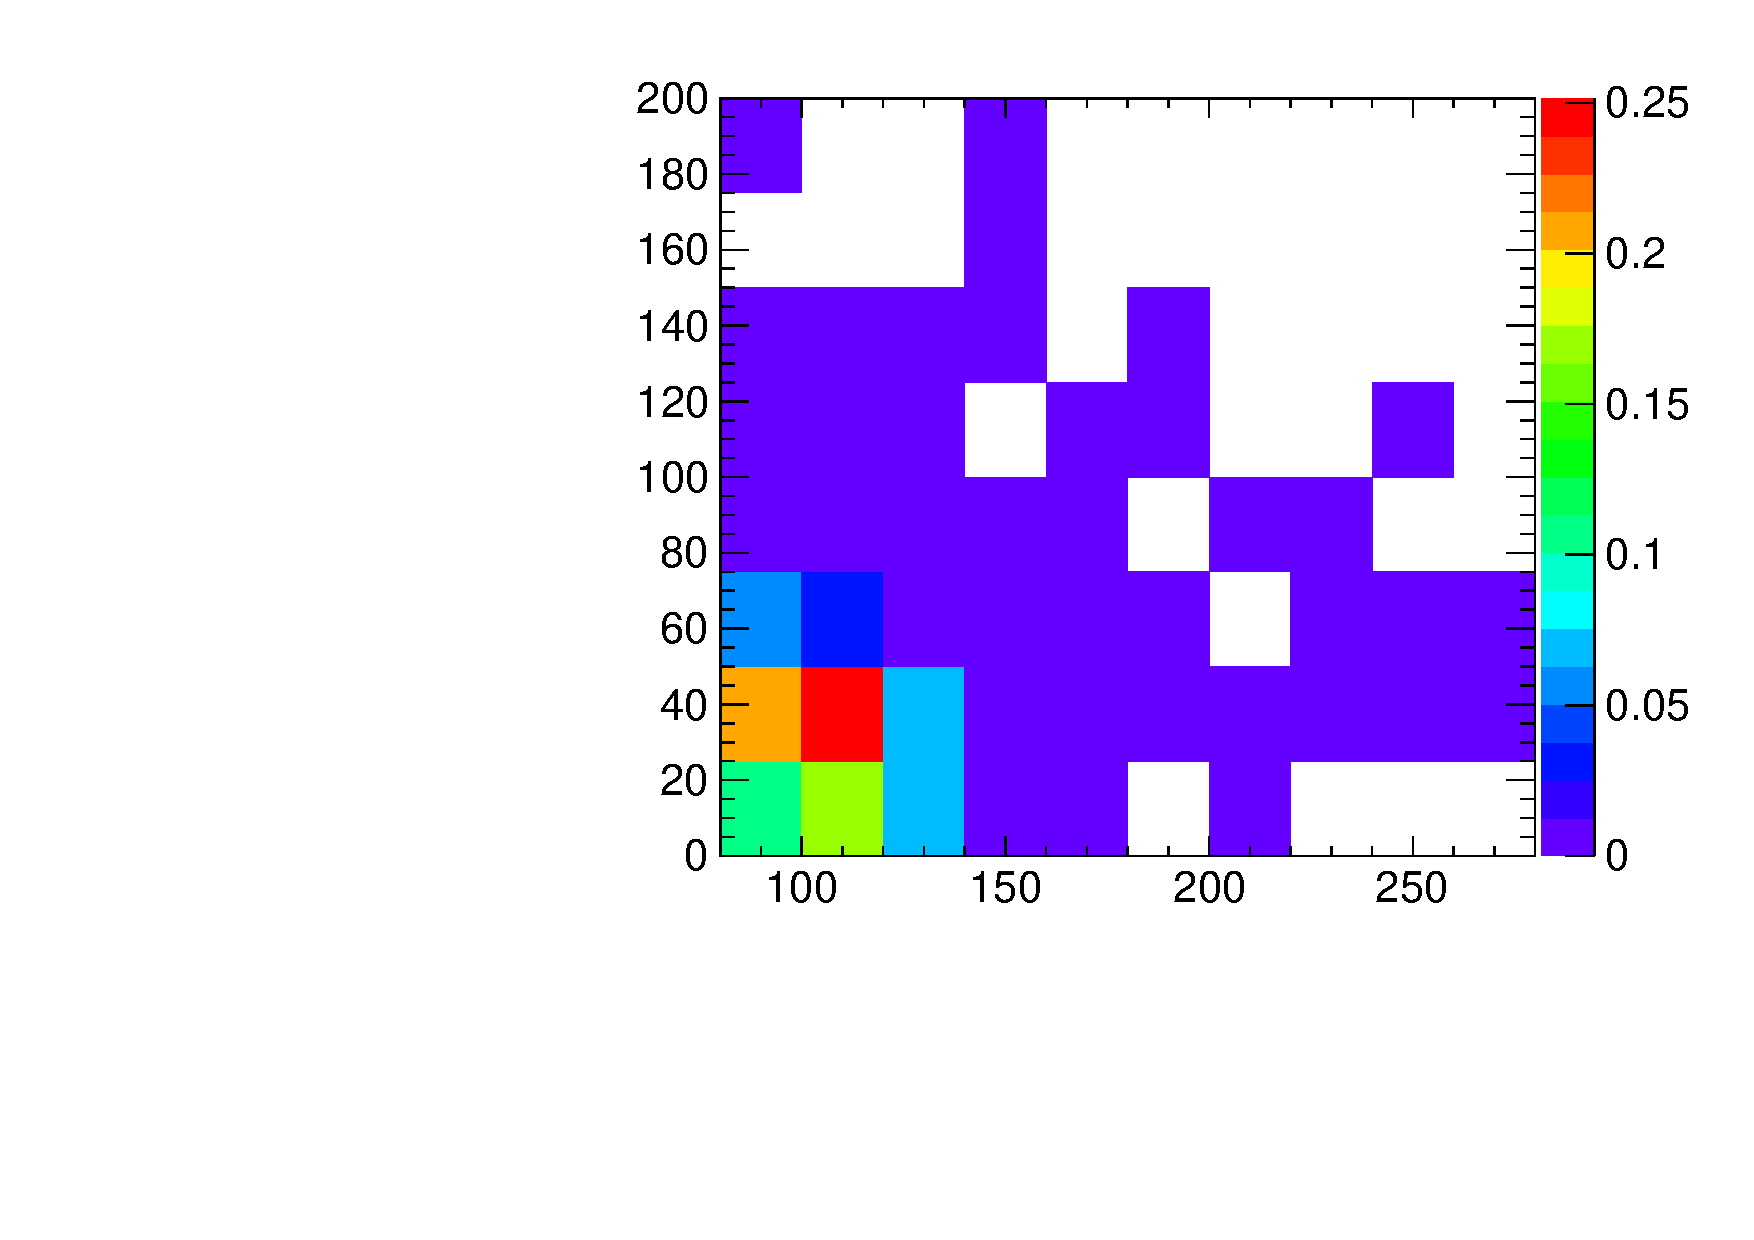
\includegraphics[width=.35\textwidth]{figures/templates/sig_2D_mH125_0j_of.pdf}
	}
	\subfigure[\qqww]{
	\centering
	\label{subfig:template_qqWW_125}
		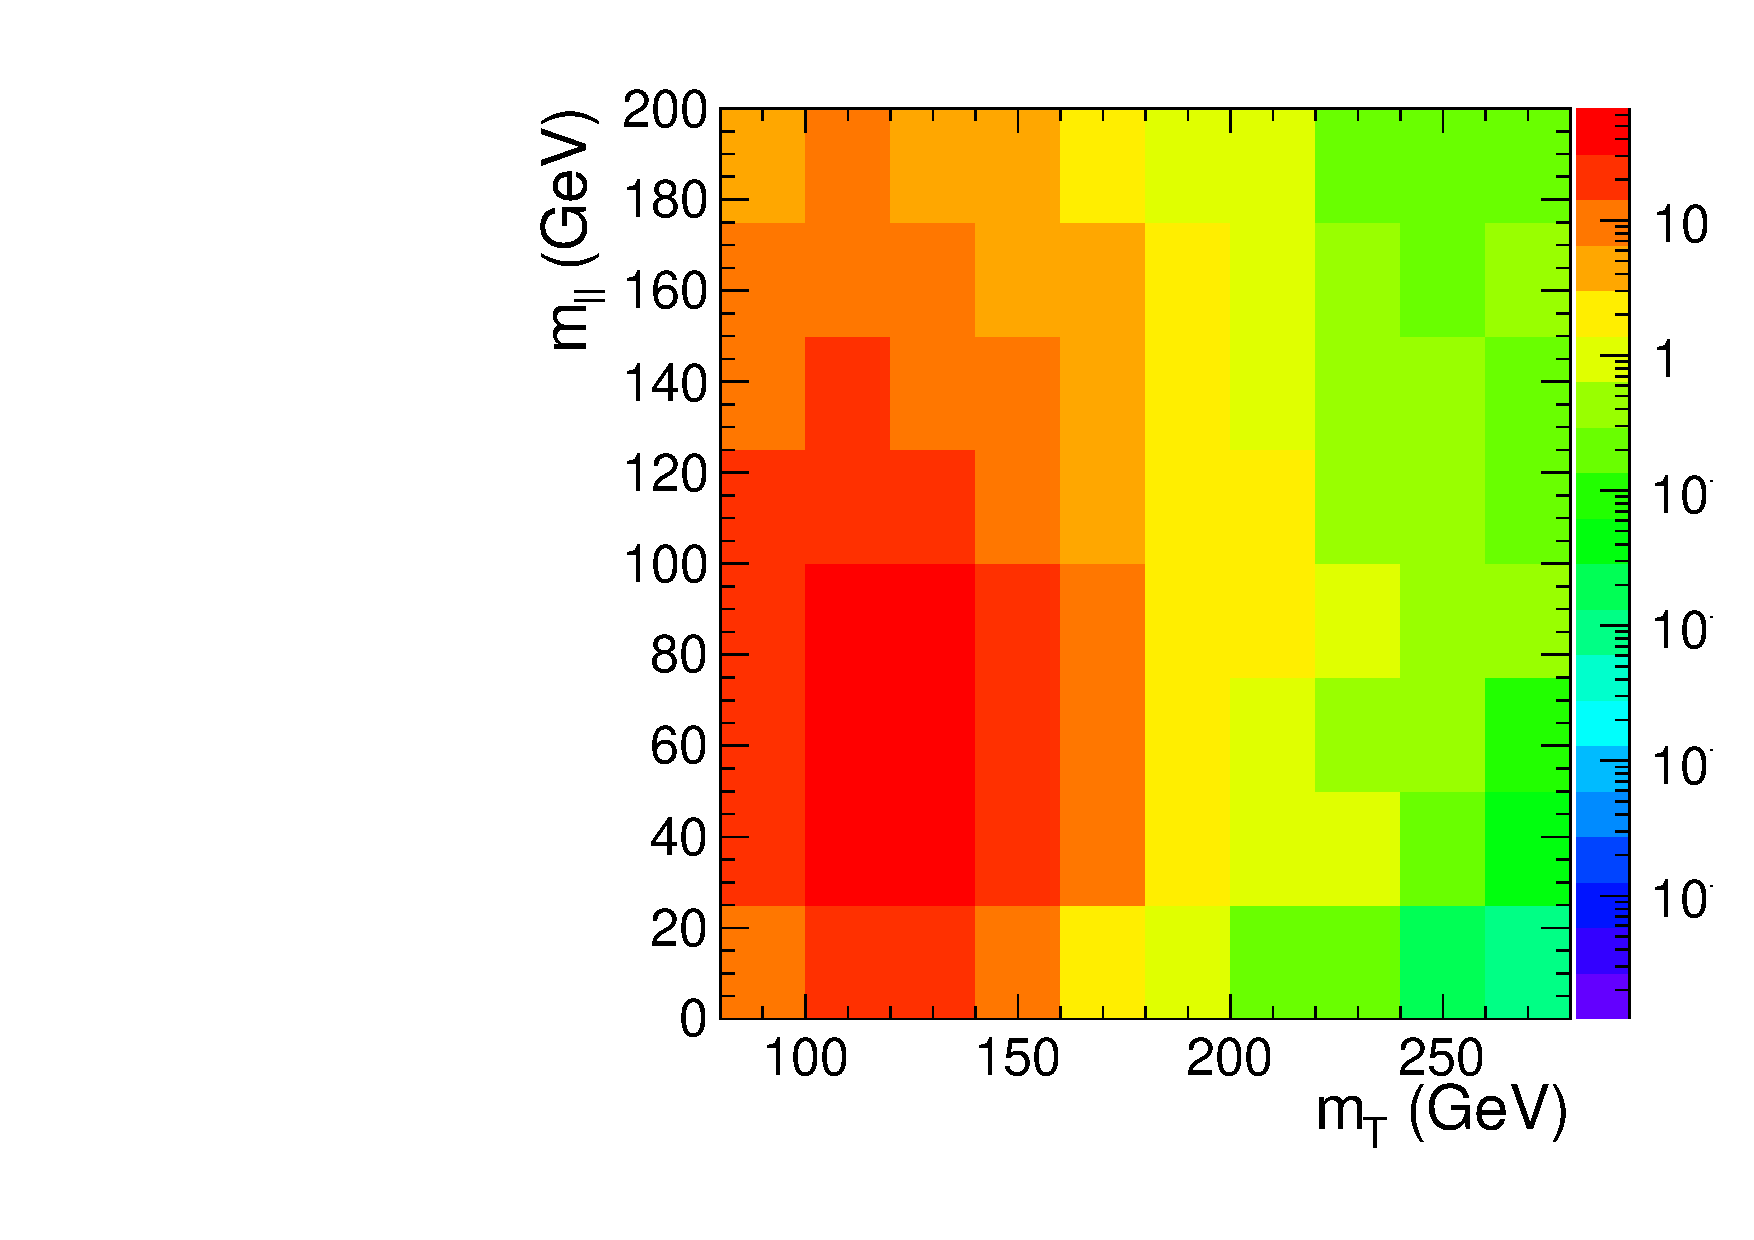
\includegraphics[width=.35\textwidth]{figures/templates/qqWW_2D_mH125_0j_of.pdf}
	}
	
	\caption{2D templates at \mHi = 125 \GeV} 
	\label{fig:templates_125_ex}

\end{figure}
	
